%%%%%%%%%%%%%%%%%%%%%%%%%%%%%
%%%%%%%% - Schedule - %%%%%%%
%%%%%%%%%%%%%%%%%%%%%%%%%%%%%
\subsection{Schedule}
\label{ssec:Schedule}
\begin{wrapfigure}[12]{R}{0pt}
		\raisebox{0pt}[\dimexpr\height-2\baselineskip\relax]{
	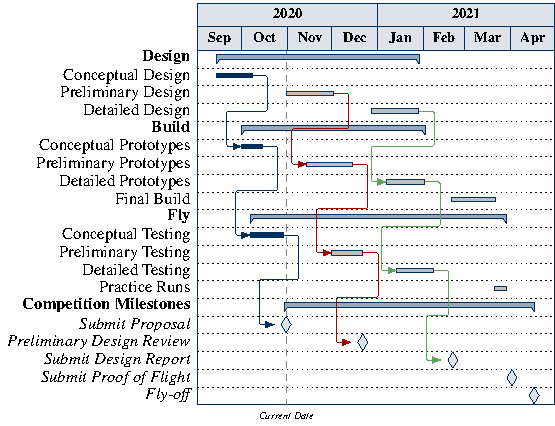
\includegraphics[width=0.45\textwidth]{ganttchart.pdf}}
	\caption{Our {\color{\BYUblue} conceptual}, {\color{\BYUred} preliminary}, and {\color{\BYUgreen} detailed} phased DBF timeline for this competition season.}
	\label{fig:plannedtiming}
\end{wrapfigure} 
%timeline description.
\Cref{fig:plannedtiming} depicts our planned timeline for the year. \Cref{sec:ManufacturingPlan,sec:TestingPlan} describe the flow of our schedule in more detail. We have completed the conceptual design presented herein and have moved on to our preliminary design phase. We also began prototyping early in order to apply a ``fail fast, fail often'' methodology to quickly fill any gaps in understanding and allow our underclassmen to develop their aircraft design intuition faster than if we waited to prototype after completing all the design phases. As shown in \cref{fig:plannedtiming}, each of our DBF phases ends with the required competition submissions and/or an internal design review.
%TODO: If room, include a photo of the latest prototype somewhere.
%timeline figure included above since it looks better there.